\documentclass{article}\usepackage[]{graphicx}\usepackage[]{color}
% maxwidth is the original width if it is less than linewidth
% otherwise use linewidth (to make sure the graphics do not exceed the margin)
\makeatletter
\def\maxwidth{ %
  \ifdim\Gin@nat@width>\linewidth
    \linewidth
  \else
    \Gin@nat@width
  \fi
}
\makeatother

\definecolor{fgcolor}{rgb}{0.345, 0.345, 0.345}
\newcommand{\hlnum}[1]{\textcolor[rgb]{0.686,0.059,0.569}{#1}}%
\newcommand{\hlstr}[1]{\textcolor[rgb]{0.192,0.494,0.8}{#1}}%
\newcommand{\hlcom}[1]{\textcolor[rgb]{0.678,0.584,0.686}{\textit{#1}}}%
\newcommand{\hlopt}[1]{\textcolor[rgb]{0,0,0}{#1}}%
\newcommand{\hlstd}[1]{\textcolor[rgb]{0.345,0.345,0.345}{#1}}%
\newcommand{\hlkwa}[1]{\textcolor[rgb]{0.161,0.373,0.58}{\textbf{#1}}}%
\newcommand{\hlkwb}[1]{\textcolor[rgb]{0.69,0.353,0.396}{#1}}%
\newcommand{\hlkwc}[1]{\textcolor[rgb]{0.333,0.667,0.333}{#1}}%
\newcommand{\hlkwd}[1]{\textcolor[rgb]{0.737,0.353,0.396}{\textbf{#1}}}%
\let\hlipl\hlkwb

\usepackage{framed}
\makeatletter
\newenvironment{kframe}{%
 \def\at@end@of@kframe{}%
 \ifinner\ifhmode%
  \def\at@end@of@kframe{\end{minipage}}%
  \begin{minipage}{\columnwidth}%
 \fi\fi%
 \def\FrameCommand##1{\hskip\@totalleftmargin \hskip-\fboxsep
 \colorbox{shadecolor}{##1}\hskip-\fboxsep
     % There is no \\@totalrightmargin, so:
     \hskip-\linewidth \hskip-\@totalleftmargin \hskip\columnwidth}%
 \MakeFramed {\advance\hsize-\width
   \@totalleftmargin\z@ \linewidth\hsize
   \@setminipage}}%
 {\par\unskip\endMakeFramed%
 \at@end@of@kframe}
\makeatother

\definecolor{shadecolor}{rgb}{.97, .97, .97}
\definecolor{messagecolor}{rgb}{0, 0, 0}
\definecolor{warningcolor}{rgb}{1, 0, 1}
\definecolor{errorcolor}{rgb}{1, 0, 0}
\newenvironment{knitrout}{}{} % an empty environment to be redefined in TeX

\usepackage{alltt}
\usepackage[]{graphicx}
\usepackage[]{color}
% maxwidth is the original width if it is less than linewidth
% otherwise use linewidth (to make sure the graphics do not exceed the margin)
\IfFileExists{upquote.sty}{\usepackage{upquote}}{}
\begin{document}

\section{Introduction}

\subsection{How is particulate matter analyzed?}

The PM sensor has several components to measure the particles in the air -- remember, we don't know what the make up of these particles might be -- but we can get an estimate of their size distribution. We have written the code to collect particles smaller than 1$\mu$m, 2.5$\mu$m and 10$\mu$m. 

Figure~\ref{fig:hpsensor} is a schematic of the particle sensor made by Honeywell (HPM Series --- Particulate Matter Sensors 32322550HP). The one we are using is made by Plantower. As a Chinese company, most of their literature is in Chinese, so I didn't find something that I could interpret for us. 

\begin{figure}
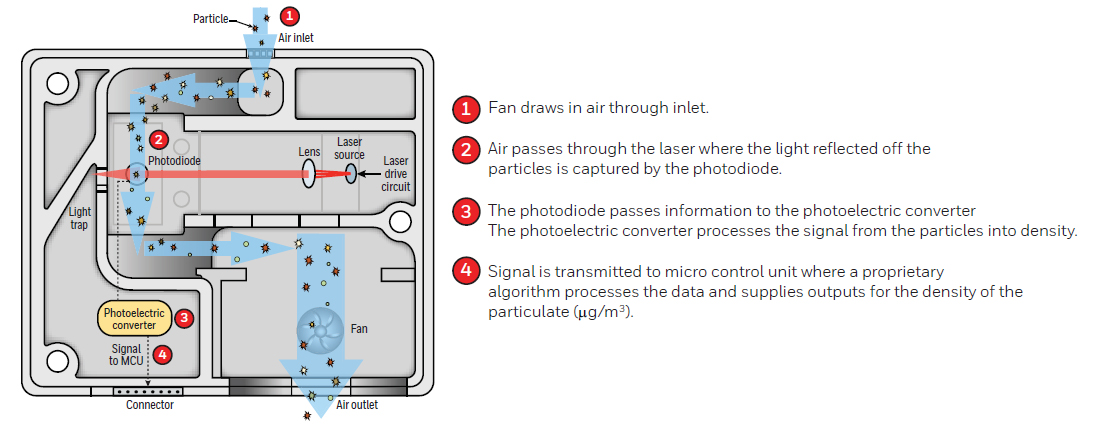
\includegraphics[width=1.00\textwidth]{images/4_SensorSchemiatic}
\caption{Schematic of Honeywell Particulate Matter Sensor. A laser light source illuminates a particle as it is pulled through the detection chamber. As particles pass through the laser beam, the light reflects off the particles and is recorded on the photo or light detector. The light is then analyzed and converted to an electrical signal to calculate particle concentration.}
\label{fig:hpsensor}
\end{figure}

Our sensors can generate several categories of PM data. Using a laser and light defraction, the number and size of the particles can be estimated (Figure~\ref{fig:defraction}).

\begin{figure}
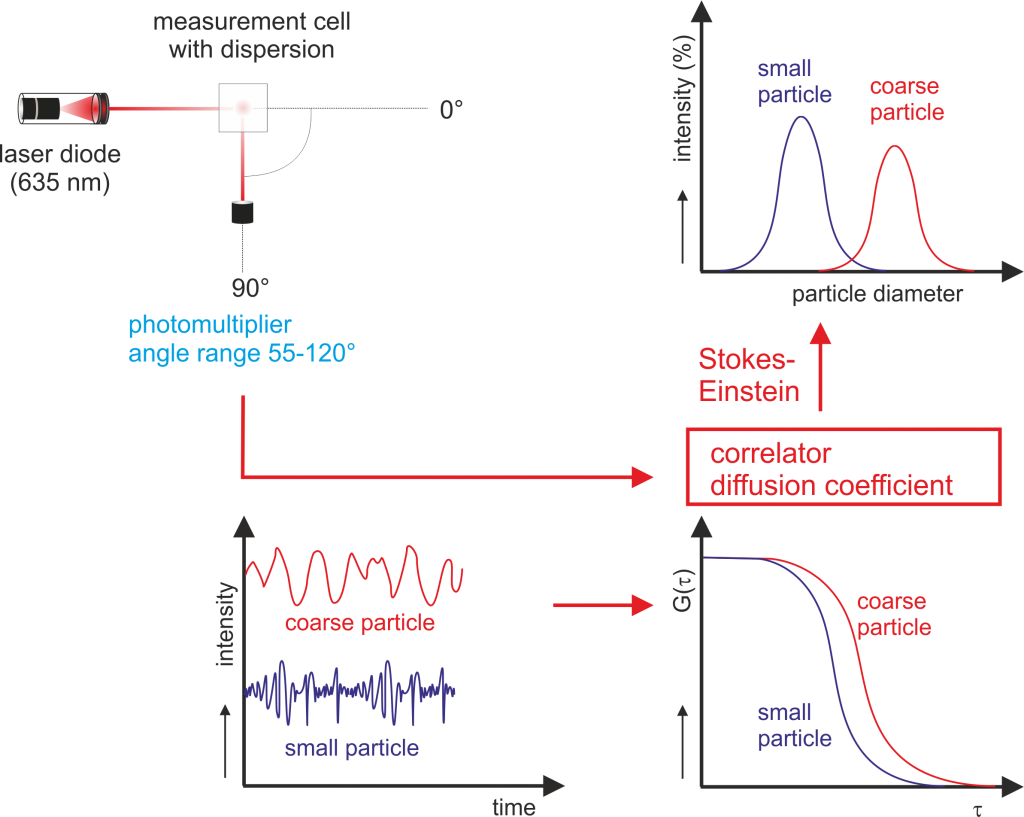
\includegraphics[width=0.70\textwidth]{images/4_Measurement-principle}
\caption{In particle size measurements using light scattering (DLS), a laser beam is scattered on very small, finely dispersed particles in a highly diluted matrix. 
The scattered light of each particle will then interfere with each other. Since the particles constantly change locations, the position of the scattering centers changes with respect to each other and the interferences lead to small fluctuations in scattering intensity (this explains the name ``dynamic'' light scattering). 
}

\label{fig:defraction}
\end{figure}

\section{Data Collection}
\subsection{What data is collected by the PMS5003?}

The PMS5003 generates the following data: 

\begin{description}
  \item[Data 1] refers to PM1.0 concentration unit $\mu$g/m$^3$(CF=1,standard particle)\footnote{The Asterisk on Data 1 and Data 4 is defined on the same page as ``Note: CF=1 should be used in the factory environment''}
  \item[Data 2] refers to PM2.5 concentration unit $\mu$g/m$^3$(CF=1,standard particle)
  \item[Data 3] refers to PM10 concentration unit $\mu$g/m$^3$(CF=1,standard particle)
  \item[Data 4] refers to PM1.0 concentration unit * $\mu$g/m$^3$(under atmospheric environment)
  \item[Data 5] refers to PM2.5 concentration unit $\mu$g/m$^3$(under atmospheric environment)
  \item[Data 6] refers to concentration unit (under atmospheric environment) $\mu$g/m$^3$
  \item[Data 7] indicates the number of particles with diameter beyond 0.3 $\mu$m in 0.1 L of air.
  \item[Data 8] indicates the number of particles with diameter beyond 0.5 $\mu$m in 0.1 L of air.
  \item[Data 9] indicates the number of particles with diameter beyond 1.0 $\mu$m in 0.1 L of air.
  \item[Data 10] indicates the number of particles with diameter beyond 2.5 $\mu$m in 0.1 L of air.
  \item[Data 11] indicates the number of particles with diameter beyond 5.0 $\mu$m in 0.1 L of air.
  \item[Data 12] indicates the number of particles with diameter beyond 10 $\mu$m in 0.1 L of air

\end{description}

The first set are labeled ``standard'', while the second set are labeled ``atmospheric environment''. What do these measure and how do the ``standard'' ones differ from the ``atmospheric environment'' ones?

It has to do with the density of the air used for calculations. "Standard" refers to the concentration ``corrected'' to the ``standard atmosphere'' which in the US is DEFINED as ``having a temperature of 288.15 K at the sea level 0 km geo-potential height and 1013.25 hPa''. NOTE: 288.15 K equals 25 C and Pa are ``pascals'' which is a meausure of pressure. 

On the other hand, the ``ambient conditions'' are just as the air is ``now'' (whatever temperature and pressure there is). Now what does that mean\ldots

Air being a gas, it is compressible which means that it changes its volume when the pressure changes so when you report concentrations as mass per volume of air it is relevant at what pressure that volume is calculated. For example, if you have a bunch of particles rising in the air in a bubble (no loss of particles, no addition, they're just riding a bubble up in the air) then, as they rise, the pressure drops so what was 1cc at the ground it is now 2cc so the concentration of what was in the bubble is now half without anything actually changing other than the ambient pressure. So, it is common to report concentrations (of anything) as ``x mg per standard m3'' and because we scientist don't like to write much (current example excluded) you'll usually see the ``standard'' being dropped because it is ``implicit''.

For gases it is also common to report concentrations as ``parts per million'' or ``ppm'' and that metric is independent of the volume of air as it represents the number of molecules of the gas in a million molecules of air (including the target gas).

In conclusion, I use the ``standard'' readings for reporting but keep the ``ambient conditions'' for analysis. I haven't used these things in high altitudes so for all my deployments the standard and ambient are very similar. I have written code to extract the standard values only -- but you can certain add the ambient if you want to see if there is a difference -- could be important if you are above 1000 ft in elevation. 
\section{Collecting the data}

\subsection{Read SD Card}

Once the data have been collected, you can extract the data from the SD card and upland to Rstudio for processing. Shut down the Pi and read the SD card to collect all of the Air\_Quality.csv files created. It might be useful to put them together using excel, but we can do that easily enough using R. 

\subsection{Processing the data}

We create a script to process the data and allow you to create a reasonably user-friendly dataframe to analyze the data.

\begin{knitrout}
\definecolor{shadecolor}{rgb}{0.969, 0.969, 0.969}\color{fgcolor}\begin{kframe}
\begin{alltt}
\hlstd{filepath.csv} \hlkwb{=} \hlstr{"/home/CAMPUS/mwl04747/github/EJnPi/data/Air_Quality.csv"}
\hlstd{rawdata} \hlkwb{=} \hlkwd{read.csv}\hlstd{(filepath.csv)}

\hlkwd{names}\hlstd{(rawdata)}\hlkwb{=} \hlkwd{c}\hlstd{(}\hlstr{"X1"}\hlstd{,} \hlstr{"X2"}\hlstd{,} \hlstr{"Month"}\hlstd{,} \hlstr{"Day"}\hlstd{,} \hlstr{"Hour"}\hlstd{,}
    \hlstr{"Minute"}\hlstd{,} \hlstr{"Second"}\hlstd{,} \hlstr{"X3"}\hlstd{,} \hlstr{"X4"}\hlstd{,} \hlstr{"pm1_cf"}\hlstd{,} \hlstr{"X5"}\hlstd{,} \hlstr{"pm25_cf"}\hlstd{,} \hlstr{"X6"}\hlstd{,}
    \hlstr{"pm10_cf"}\hlstd{,} \hlstr{"X7"}\hlstd{,} \hlstr{"pm1"}\hlstd{,} \hlstr{"X8"}\hlstd{,} \hlstr{"pm25"}\hlstd{,} \hlstr{"pm10."}\hlstd{,} \hlstr{"X9"}\hlstd{)}

\hlstd{rawdata}\hlopt{$}\hlstd{pm1_cf} \hlkwb{=} \hlkwd{as.numeric}\hlstd{(}\hlkwd{gsub}\hlstd{(}\hlstr{'[)]'}\hlstd{,} \hlstr{''}\hlstd{, rawdata}\hlopt{$}\hlstd{pm1_cf))}
\hlstd{rawdata}\hlopt{$}\hlstd{pm25_cf} \hlkwb{=} \hlkwd{as.numeric}\hlstd{(}\hlkwd{gsub}\hlstd{(}\hlstr{'[)]'}\hlstd{,} \hlstr{''}\hlstd{, rawdata}\hlopt{$}\hlstd{pm25_cf))}
\hlstd{rawdata}\hlopt{$}\hlstd{pm10_cf} \hlkwb{=} \hlkwd{as.numeric}\hlstd{(}\hlkwd{gsub}\hlstd{(}\hlstr{'[)]'}\hlstd{,} \hlstr{''}\hlstd{, rawdata}\hlopt{$}\hlstd{pm10_cf))}
\hlkwd{as.Date}\hlstd{(}\hlkwd{with}\hlstd{(rawdata,} \hlkwd{paste}\hlstd{(}\hlstr{"2020"}\hlstd{, Month, Day,}\hlkwc{sep}\hlstd{=}\hlstr{"-"}\hlstd{)),} \hlstr{"%Y-%m-%d"}\hlstd{)}
\end{alltt}
\begin{verbatim}
## [1] "2020-10-18" "2020-10-18" "2020-10-18" "2020-10-18" "2020-10-18"
## [6] "2020-10-18" "2020-10-18" "2020-10-18"
\end{verbatim}
\begin{alltt}
\hlkwd{library}\hlstd{(lubridate)}
\end{alltt}


{\ttfamily\noindent\itshape\color{messagecolor}{\#\# \\\#\# Attaching package: 'lubridate'}}

{\ttfamily\noindent\itshape\color{messagecolor}{\#\# The following object is masked from 'package:base':\\\#\# \\\#\#\ \ \ \  date}}\begin{alltt}
\hlstd{rawdata}\hlopt{$}\hlstd{DateTime} \hlkwb{=} \hlkwd{with}\hlstd{(rawdata,} \hlkwd{ymd_hms}\hlstd{(}\hlkwd{paste}\hlstd{(}\hlstr{"2020"}\hlstd{, Month, Day, Hour, Minute, Second,} \hlkwc{sep}\hlstd{=} \hlstr{'-'}\hlstd{)))}
\end{alltt}


{\ttfamily\noindent\color{warningcolor}{\#\# Warning:\ \ 4 failed to parse.}}\begin{alltt}
\hlkwd{head}\hlstd{(rawdata)}
\end{alltt}
\begin{verbatim}
##                         X1                      X2 Month Day Hour Minute Second
## 1 OrderedDict([('DateTime'  datetime.datetime(2020    10  18   21     27     31
## 2 OrderedDict([('DateTime'  datetime.datetime(2020    10  18   22     27     41
## 3 OrderedDict([('DateTime'  datetime.datetime(2020    10  18   23     27     21
## 4 OrderedDict([('DateTime'  datetime.datetime(2020    10  18   24     27     31
## 5 OrderedDict([('DateTime'  datetime.datetime(2020    10  18   25     27     41
## 6 OrderedDict([('DateTime'  datetime.datetime(2020    10  18   26     27     21
##          X3         X4 pm1_cf          X5 pm25_cf          X6 pm10_cf      X7
## 1  546422))  ('pm1_cf'      9  ('pm25_cf'      15  ('pm10_cf'      17  ('pm1'
## 2  910120))  ('pm1_cf'     11  ('pm25_cf'      14  ('pm10_cf'      12  ('pm1'
## 3  185161))  ('pm1_cf'     13  ('pm25_cf'      14  ('pm10_cf'      16  ('pm1'
## 4  546422))  ('pm1_cf'     12  ('pm25_cf'      15  ('pm10_cf'      19  ('pm1'
## 5  910120))  ('pm1_cf'      9  ('pm25_cf'      14  ('pm10_cf'      16  ('pm1'
## 6  185161))  ('pm1_cf'     11  ('pm25_cf'      18  ('pm10_cf'      16  ('pm1'
##   pm1       X8 pm25    pm10.     X9            DateTime
## 1  9)  ('pm25'  15)  ('pm10'  17)]) 2020-10-18 21:27:31
## 2  9)  ('pm25'  14)  ('pm10'  16)]) 2020-10-18 22:27:41
## 3  9)  ('pm25'  14)  ('pm10'  16)]) 2020-10-18 23:27:21
## 4  9)  ('pm25'  15)  ('pm10'  17)]) 2020-10-19 00:27:31
## 5  9)  ('pm25'  14)  ('pm10'  16)])                <NA>
## 6  9)  ('pm25'  14)  ('pm10'  16)])                <NA>
\end{verbatim}
\begin{alltt}
\hlcom{# Remove Variables}
\hlstd{cleandata} \hlkwb{=} \hlkwd{subset}\hlstd{(rawdata,} \hlkwc{select}\hlstd{=}\hlkwd{c}\hlstd{(DateTime, pm1_cf, pm25_cf, pm10_cf))}
\end{alltt}
\end{kframe}
\end{knitrout}

\subsection{Plot Data}

\begin{knitrout}
\definecolor{shadecolor}{rgb}{0.969, 0.969, 0.969}\color{fgcolor}\begin{kframe}
\begin{alltt}
\hlkwd{hist}\hlstd{(cleandata}\hlopt{$}\hlstd{pm25_cf)}
\end{alltt}
\end{kframe}
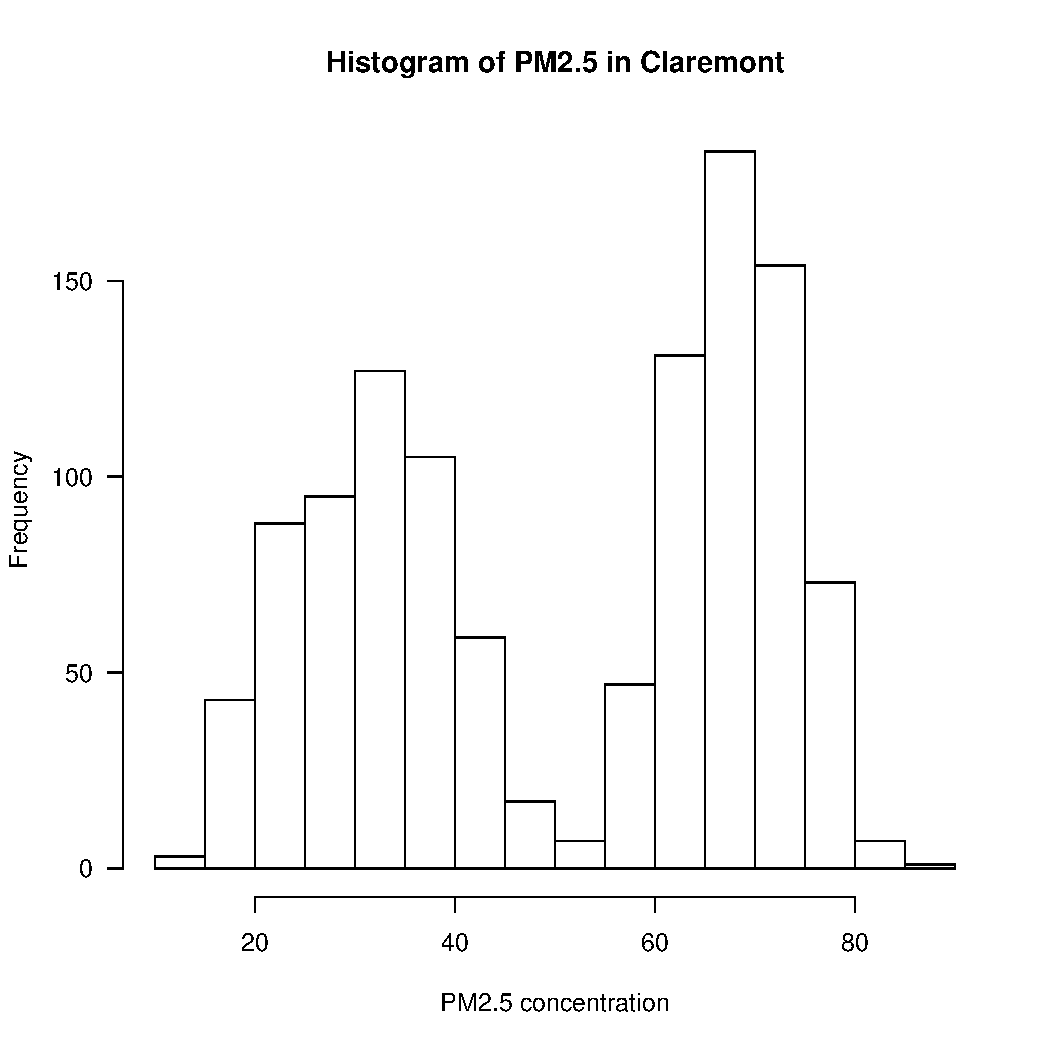
\includegraphics[width=\maxwidth]{figure/unnamed-chunk-2-1} 

\end{knitrout}


\section{Comparing Data to EPA Stations}

\subsection{Using previous collected data}



\subsection{Comparing $\mu$ to EPA Data}

The population mean (monthly average from the EPA data) is a parameter estimate. We can determine if the values you collected fall within the parameter estimate and it's 95\% confidence intervals. 


\subsection{More Intricate Analysis}

You could look to see if the there is a different during the time of the day or day of the week. You could move you sensor around in and outside your house and see if air quality is better / worse or the same\ldots.

We can help you with r code if you'd like to follow up with these additional questions. 


\end{document}
